\documentclass[12pt]{article}%
\usepackage{amsfonts}
\usepackage{fancyhdr}
\usepackage{comment}
\usepackage[letterpaper, top=2.5cm, bottom=2.5cm, left=2.2cm, right=2.2cm]%
{geometry}
\usepackage{times}
\usepackage{amsmath}
\usepackage{changepage}
\usepackage{multirow}
\usepackage{amssymb}
\usepackage{graphicx}%
\graphicspath{ {images/} }
\usepackage{amsmath}
\setcounter{MaxMatrixCols}{30}
\newtheorem{theorem}{Theorem}
\newtheorem{acknowledgement}[theorem]{Acknowledgement}
\newtheorem{algorithm}[theorem]{Algorithm}
\newtheorem{axiom}{Axiom}
\newtheorem{case}[theorem]{Case}
\newtheorem{claim}[theorem]{Claim}
\newtheorem{conclusion}[theorem]{Conclusion}
\newtheorem{condition}[theorem]{Condition}
\newtheorem{conjecture}[theorem]{Conjecture}
\newtheorem{corollary}[theorem]{Corollary}
\newtheorem{criterion}[theorem]{Criterion}
\newtheorem{definition}[theorem]{Definition}
\newtheorem{example}[theorem]{Example}
\newtheorem{exercise}[theorem]{Exercise}
\newtheorem{lemma}[theorem]{Lemma}
\newtheorem{notation}[theorem]{Notation}
\newtheorem{problem}[theorem]{Problem}
\newtheorem{proposition}[theorem]{Proposition}
\newtheorem{remark}[theorem]{Remark}
\newtheorem{solution}[theorem]{Solution}
\newtheorem{summary}[theorem]{Summary}
\newenvironment{proof}[1][Proof]{\textbf{#1.} }{\ \rule{0.5em}{0.5em}}

\newcommand{\Q}{\mathbb{Q}}
\newcommand{\R}{\mathbb{R}}
\newcommand{\C}{\mathbb{C}}
\newcommand{\Z}{\mathbb{Z}}

\newcommand*{\pd}[3][]{\ensuremath{\frac{\partial^{#1} #2}{\partial #3}}}

\usepackage{enumerate}
\usepackage{array}
\newcolumntype{M}{>{$}c<{$}}


\begin{document}

\title{CS 440/ECE448 Homework 4}
\author{Tanishq Dubey (tdubey3)}
\date{\today}
\maketitle
\section*{Problem 1}
    \begin{enumerate}[1.]
            \item
                $\textbf{P}(\neg a) = $
                \[0.05 + 0.10 + 0.15 + 0.15\]
                \[0.45\]
            \item
                $\textbf{P}(B) = $
                \begin{center}
                    $P(b) = 0.20 + 0.10 + 0.05 + 0.10$. \\
                    $P(b) = 0.45$. \\
                    $P(\neg b) = 0.10 + 0.15 + 0.15 + 0.15$ \\
                    $P(\neg b) = .55$.\\
                    $P(b) + P(\neg b) = 1$
                \end{center}
            \item
                $\textbf{P}(A|b) = $ \\
                $P(A)$ is 
                \[P(a) = 0.20 + 0.15 + 0.10 + 0.15\]
                \[P(a) = 0.55\]
                \[P(\neg a) = 0.15 + 0.15 + 0.10 + 0.05\]
                \[P(\neg a) = 0.45\]
                \[P(\neg a) + P(a) = 1\]
                And we can calculate the probability of $P(x|y)$ as $\frac{P(xy)}{P(y)}$. Thus we can say:\\
                \[ \frac{P(ab)}{P(b)} = \frac{0.3}{0.45} = \frac{2}{3}\]
                \[ \frac{P(\neg a b)}{b} = \frac{0.15}{0.45} = \frac{1}{3}\]
    \end{enumerate}
\newpage

\section*{Problem 2}
    \begin{enumerate}[1.]
        \item
            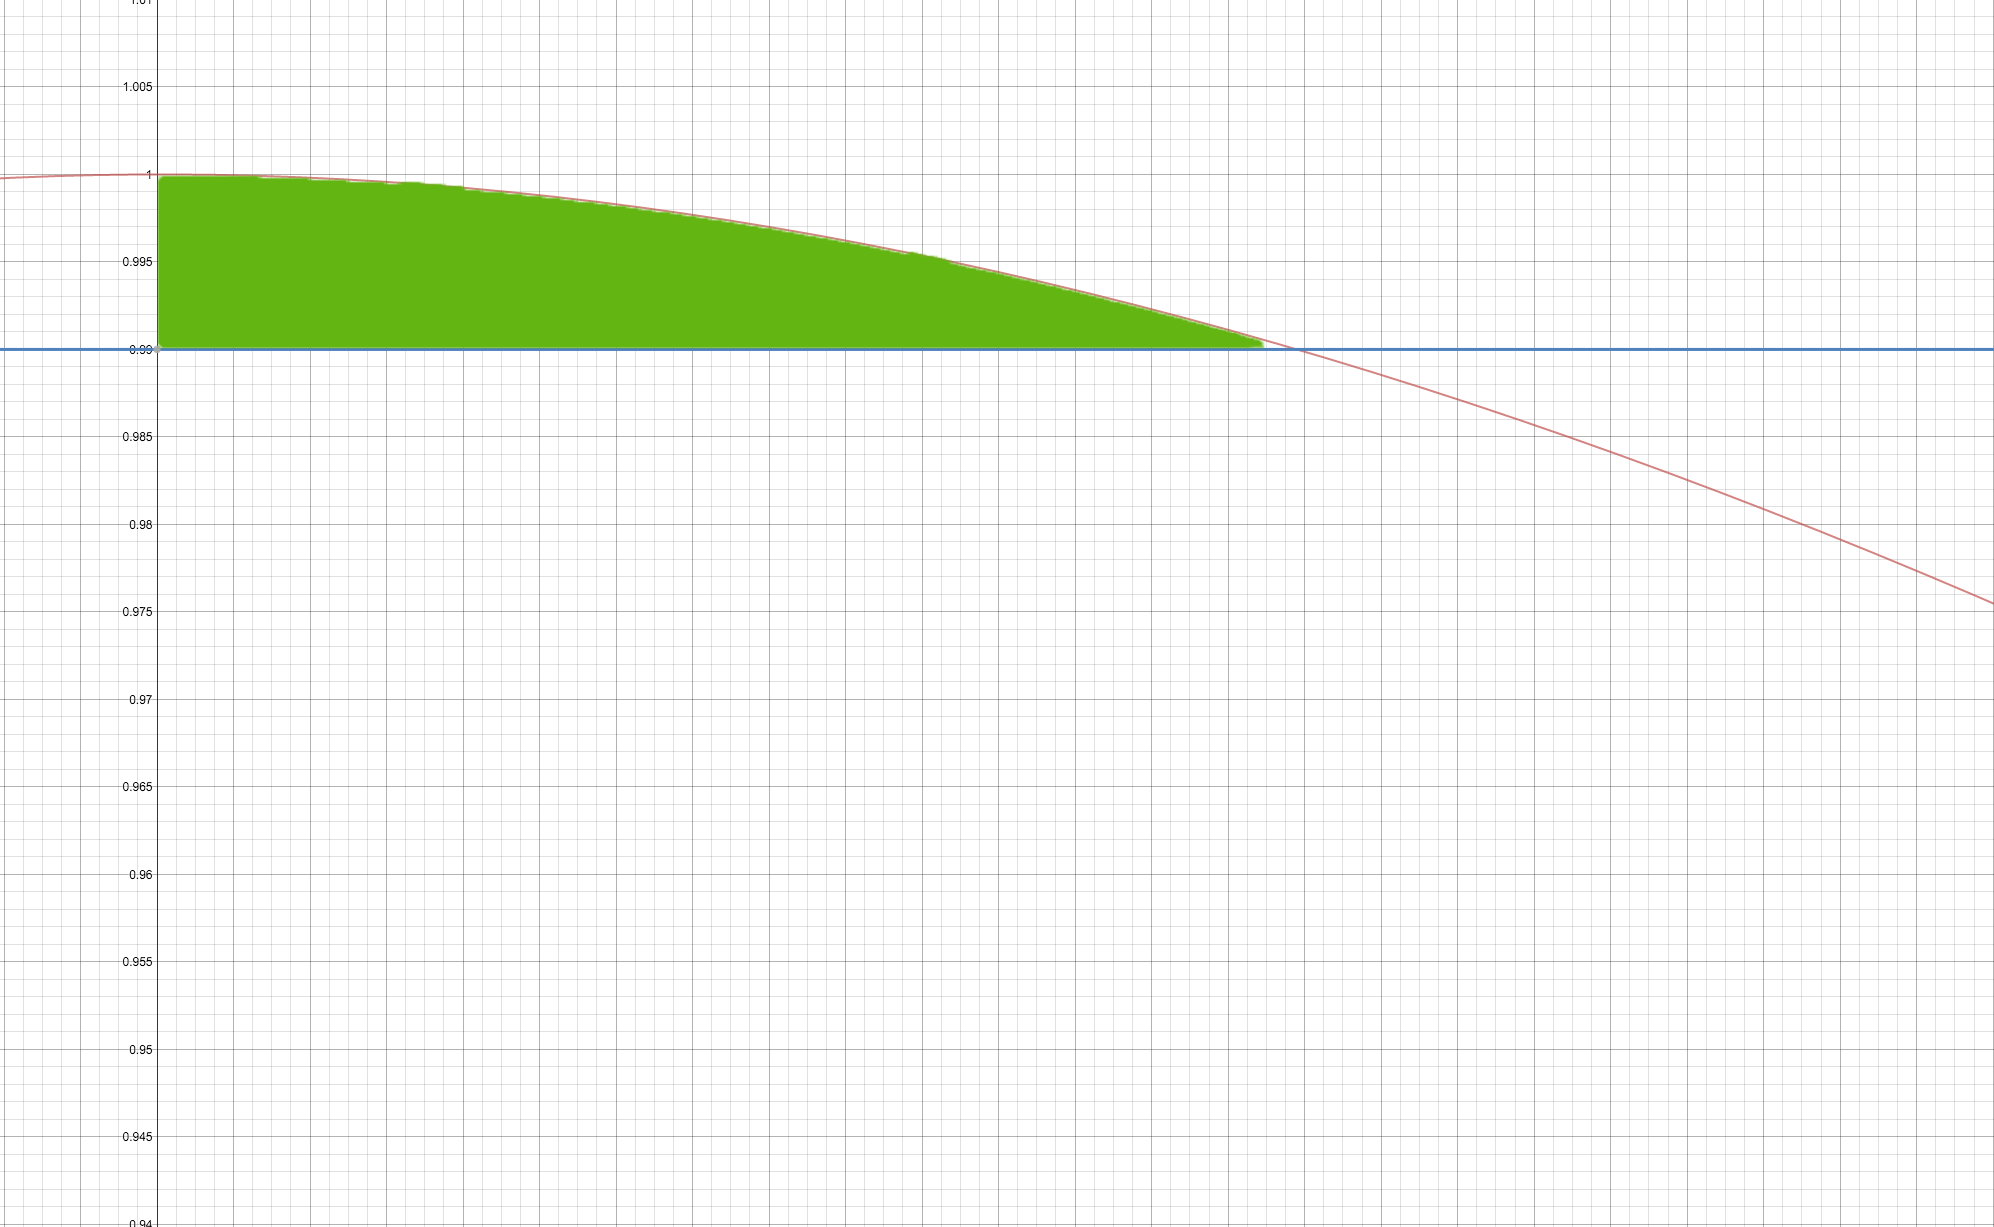
\includegraphics[scale=.25]{graphone}
        \item
            To find the value of $n$, simply find the intersect of the two lines graphed above. This value is: 148 bags.
    \end{enumerate}
    
\section*{Problem 3}
    It is known that Bayes' Theorem states:
    \[P(A|B) = \frac{P(B|A)P(A)}{P(B)}\]
    This can equally be represented as:
    \[P(A|B) = \frac{P(B|A)P(A)}{P(B|A)P(A)+P(B|\neg A)P(\neg A)}\]
    We have also been given information stating that:
    \[P(Predicted|Rain) = 0.99\]
    and
    \[P(Predicted|\neg Rain) = 0.01\]
    Thus we can say:
    \[P(Rain|Prediction) = \frac{P(Prediction|Rain)P(Rain)}{P(Prediction|Rain)P(Rain)+P(Prediction|\neg Rain)P(\neg Rain)}\]
    Thus:
    \[P(Rain|Prediction) = \frac{0.99 * \frac{1}{10000}}{0.99 * \frac{1}{10000} + 0.01 + \frac{9999}{10000}}\]
    \[P(Rain|Prediction) = 0.9804\%\]

\section*{Problem 4}
    Supposing that $P(A,B|C) = P(A|C|)P(B|C)$, it can be said:
    \[P(A,B|C) = 'P(A|C)P(B|C)\]
    \[\frac{P(A,B,C)}{P(C)} = 'P(A|C)P(B|C)\]
    \[\frac{P(A|B,C)P(B,C)}{P(C)} = 'P(A|C)P(B|C)\]
    \[\frac{P(A|B,C)P(B,C)P(C)}{P(C)} = 'P(A|C)P(B|C)\]
    \[P(A|B,C)P(B,C) = 'P(A|C)P(B|C)\]
    Hence:
    \[P(A|B,C) = 'P(A|C)\]
\end{document}